% ============================================================
% DIAGRAM: Neocognitron (1980)
% ============================================================
% Caption: Figure 3.2: Neocognitron hierarchical architecture.
%          (Adapted from Fukushima, 1980, p. 194)
% ============================================================

\documentclass[tikz,border=10pt]{standalone}
\usepackage{tikz}
\usepackage{amsmath}
\usepackage{amsfonts}

\usetikzlibrary{shapes,arrows,positioning,fit,calc,backgrounds}

\begin{document}

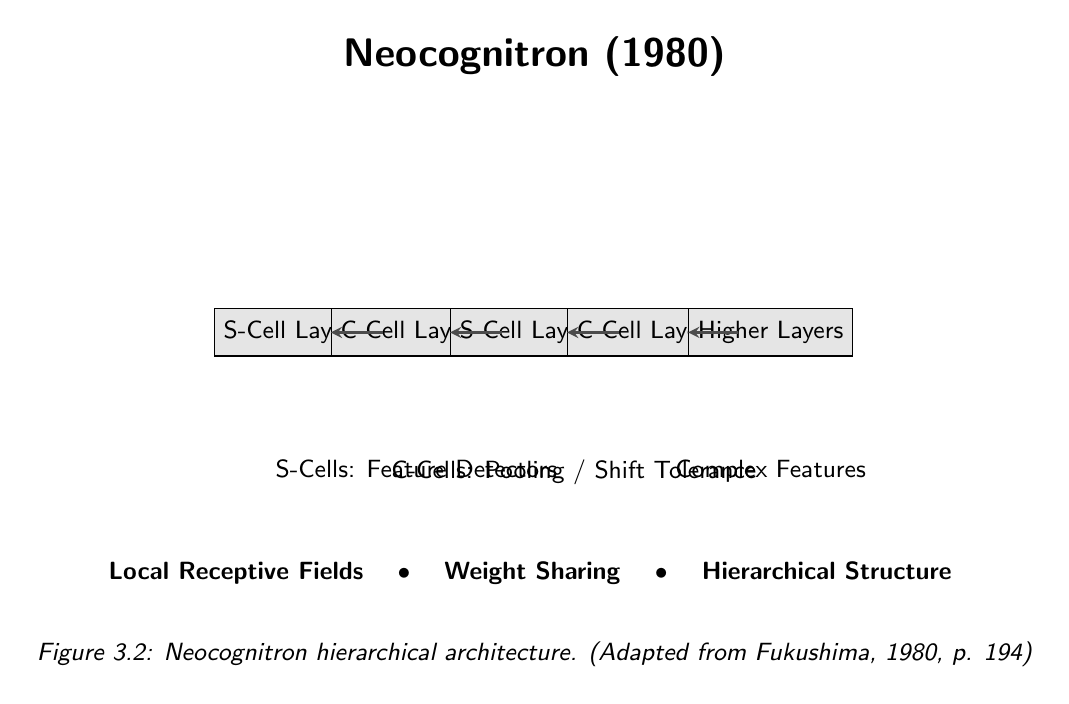
\begin{tikzpicture}[
    cell/.style={draw, rectangle, minimum width=0.8cm, minimum height=0.8cm, fill=blue!10},
    layer/.style={draw, rectangle, minimum width=1.2cm, minimum height=0.6cm, fill=gray!20, font=\sffamily\small},
    edge/.style={-stealth, thick, draw=black!70},
    label/.style={font=\sffamily\small},
    title/.style={font=\sffamily\Large\bfseries},
    caption/.style={font=\sffamily\small\itshape},
]

\node[title] at (0, 3.5) {Neocognitron (1980)};

% Hierarchy
\node[layer] (s1) at (-3, 0) {S-Cell Layer 1};
\node[layer] (c1) at (-1.5, 0) {C-Cell Layer 1};
\node[layer] (s2) at (0, 0) {S-Cell Layer 2};
\node[layer] (c2) at (1.5, 0) {C-Cell Layer 2};
\node[layer] (s3) at (3, 0) {Higher Layers};

\draw[edge] (s1) -- (c1);
\draw[edge] (c1) -- (s2);
\draw[edge] (s2) -- (c2);
\draw[edge] (c2) -- (s3);

% Explanations
\node[align=center, font=\sffamily\small, anchor=north] at (-1.5, -1.5) {S-Cells: Feature Detectors};
\node[align=center, font=\sffamily\small, anchor=north] at (0.5, -1.5) {C-Cells: Pooling / Shift Tolerance};
\node[align=center, font=\sffamily\small, anchor=north] at (3, -1.5) {Complex Features};

% Key concepts
\node[align=center, font=\sffamily\small, anchor=north] at (0, -2.8) {
  \textbf{Local Receptive Fields} \quad $\bullet$ \quad \textbf{Weight Sharing} \quad $\bullet$ \quad \textbf{Hierarchical Structure}
};

\node[caption, anchor=north] at (0, -3.8) {
  Figure 3.2: Neocognitron hierarchical architecture. (Adapted from Fukushima, 1980, p. 194)
};

\end{tikzpicture}
\end{document}
